Dans le but de concrétiser cette approche, on
s'est inspiré d'un modèle\footnote{présenté dans le Ch. 4 du travail réalisé par
\mbox{Guillaume} \mbox{Tisserant} et son équipe}, présenté sur la
figure~\ref{modele_original}, qui représente une vision du fonctionnement que
pourrait avoir une conscience artificielle. En se servant des travaux comme ceux
de Freud et de Laborit, il permet de représenter la plupart des caractéristiques
d’une conscience humaine.

\begin{figure}[H] 
\centering
FIXME FIXME FIXME
%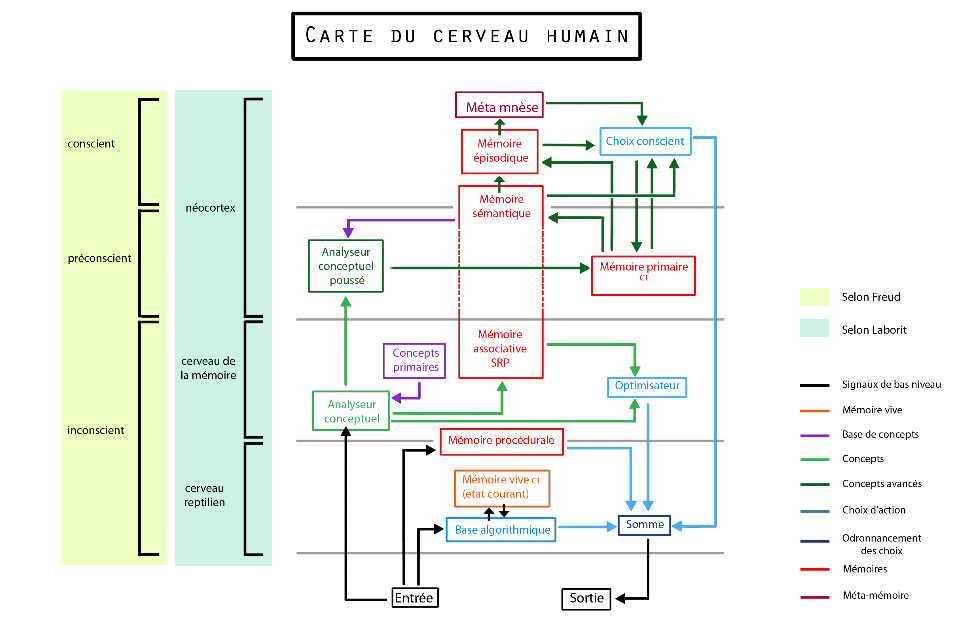
\includegraphics[width=\textwidth]{files/modele_original} 
\caption{Schéma du modèle de représentation de la conscience} 
\label{modele_original}
\end{figure}

\section{Description détaillée du modèle}
Ce modèle peut se voir comme un empilement de couches
\subsection{L’inconscient}
L'inconscient consiste du cerveau reptilien et du cerveau de la mémoire.
\subsection{Le Néocortex : la préconscience et la conscience}

\section{Synthèse}
